\chapter{Marco teórico}

\section{Estructura estelar Newtoniana}

\begin{equation}
    M ( r ) = \int _ { 0 } ^ { r } 4 \pi r ^ { 2 } \rho d r ; \quad d M ( r ) = 4 \pi r ^ { 2 } \rho d r
\end{equation}

\begin{equation}
    \frac { d P } { d r } = - \frac { G M ( r ) } { r ^ { 2 } } \rho
\end{equation}

\section{Estructura estelar relativista}

\begin{equation}
\mathrm { d } s ^ { 2 } = e ^ { 2 \nu ( r ) } \mathrm { d } t ^ { 2 } - e ^ { 2 \lambda ( r ) } \mathrm { d } r ^ { 2 } - r ^ { 2 } \left( \mathrm { d } \theta ^ { 2 } + \sin ^ { 2 }  \theta  \mathrm { d } \phi ^ { 2 } \right)    
\end{equation}

\begin{equation}
    G _ { \mu } ^ { \nu } = R _ { \mu } ^ { \nu } - \frac { 1 } { 2 } g _ { \mu } ^ { \nu } R = 8 \pi T _ { \mu } ^ { \nu }
\end{equation}

\begin{equation}
    \begin{array} { c } { T ^ { \mu \nu } = - P g ^ { \mu \nu } + ( P + \rho ) u ^ { \mu } u ^ { \nu } } \\ { g _ { \mu \nu } u ^ { \mu } u ^ { \nu } = 1 } \end{array}
\end{equation}

\begin{equation}
    T _ { 0 } ^ { 0 } = \rho(r) , \quad T _ { i } ^ { i } = - P(r)
\end{equation}

\begin{equation}
    \begin{array} { l } { G _ { 0 } ^ { 0 } = e ^ { - 2 \lambda } \left( \frac { 1 } { r ^ { 2 } } - \frac { 2 \lambda ^ { \prime } } { r } \right) - \frac { 1 } { r ^ { 2 } } = - 8 \pi  \rho ( r ) } \\ { G _ { 1 } ^ { 1 } = e ^ { - 2 \lambda } \left( \frac { 1 } { r ^ { 2 } } + \frac { 2 \nu ^ { \prime } } { r } \right) - \frac { 1 } { r ^ { 2 } } = 8 \pi  P ( r ) } \\ { G _ { 2 } ^ { 2 } = e ^ { - 2 \lambda } \left( \nu ^ { \prime \prime } + \nu ^ { \prime 2 } - \lambda ^ { \prime } \nu ^ { \prime } + \frac { \nu ^ { \prime } - \lambda ^ { \prime } } { r } \right) = 8 \pi  P ( r ) } \\ { G _ { 3 } ^ { 3 } = G _ { 2 } ^ { 2 } = 8 \pi  P ( r ) } \end{array}
\end{equation}

\begin{equation}
    \frac { d P } { d r } = - \frac { [ P ( r ) + \rho ( r ) ] \left[ M ( r ) + 4 \pi r ^ { 3 } P ( r ) \right] } { r [ r - 2 M ( r ) ] }
\end{equation}

\begin{equation}
    M ( r ) \equiv 4 \pi \int _ { 0 } ^ { r } \rho ( r ) r ^ { 2 } d r
\end{equation}

\begin{equation}
    \frac { \mathrm { d } m } { \mathrm { d } r } = 4 \pi r ^ { 2 } \rho(r)
\end{equation}

\section{Estructura interna de objetos compactos y ecuaciones de estado}

\begin{figure}[H]
    \centering
    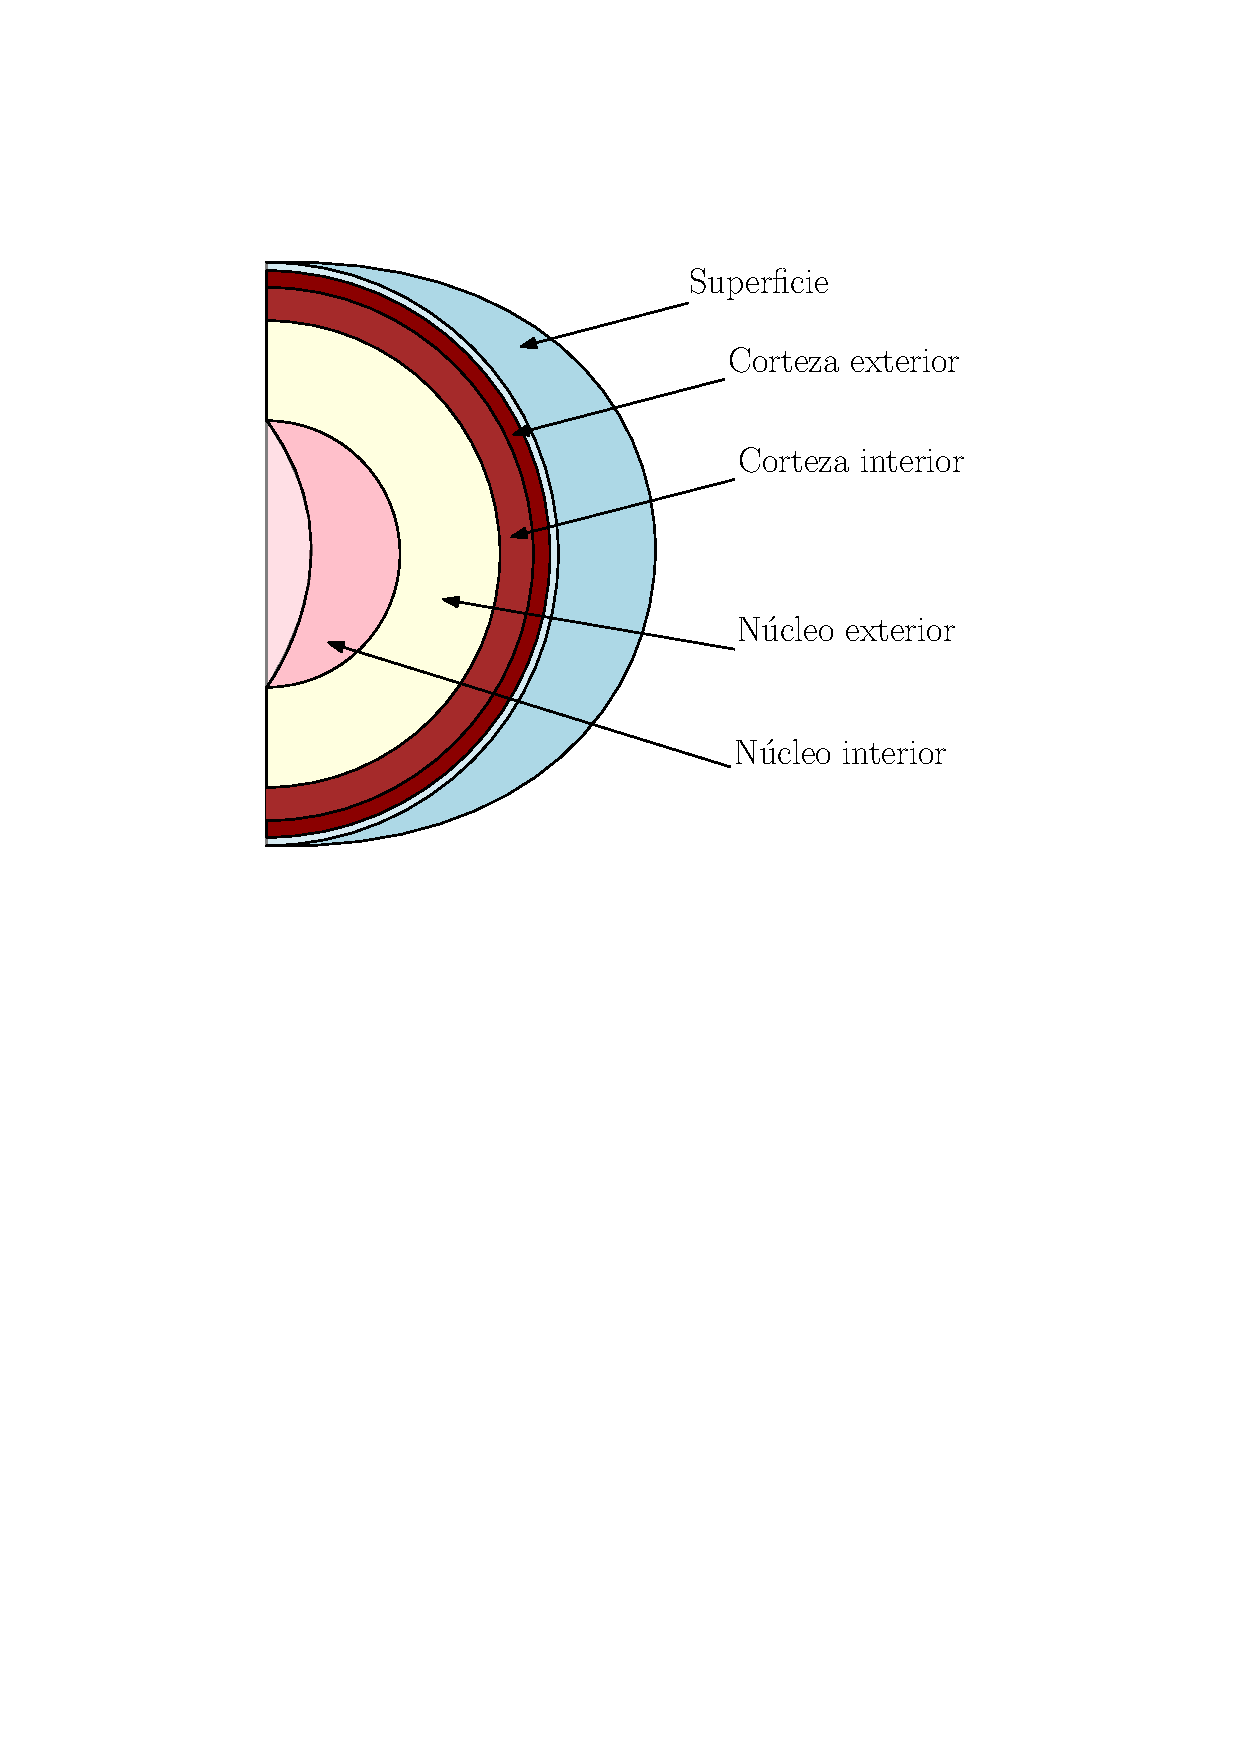
\includegraphics[width=200pt]{figures/neutronstar.pdf}
    \caption{Estructura interna de una estrella de neutrones}
    \label{NSS}
\end{figure}

\section{Criterios de estabilidad}

\subsection{Condición de estabilidad de Harrison-Zeldovich-Novikov}

\begin{equation}
    \frac { \partial M \left( \rho _ { c } \right) } { \partial \rho _ { c } } > 0
\end{equation}


\subsection{Condición de estabilidad de convección adiabática}

\begin{equation}
    \rho ^ { \prime \prime } ( r ) \leq 0
\end{equation}
